\documentclass[12pt]{article}
\usepackage[margin=1in]{geometry}
\usepackage{parskip}
\usepackage{listings}
\usepackage{xcolor}
\usepackage{url}
\usepackage{tikz}
\usetikzlibrary{arrows.meta,positioning}

\lstset{
    basicstyle=\ttfamily\small,
    breaklines=true,
    frame=single,
    backgroundcolor=\color{gray!5},
    numbers=left,
    numberstyle=\tiny\color{gray},
    numbersep=5pt,
    tabsize=2
}

\title{\textbf{CS 271 Project Report} \\[0.3em]
\large Learning State Transitions in Key-Value Logs for Anomaly Detection}

\author{
\begin{tabular}{c}
Satheesh Kumar G R \\
\texttt{satheeshkumar.geetharavi@sjsu.edu} \\
San Jos\'{e} State University
\end{tabular}
}

\begin{document}
\maketitle

\section{The Problem (Introduction)}

Modern systems generate large volumes of logs that capture system behavior using key-value pairs (e.g., service, status, latency, retry count). These logs provide detailed information about how a system evolves over time. Engineers typically analyze them using dashboards or queries by selecting specific keys.

This approach does not scale well. Anomalies in real systems are often not caused by a single field exceeding a threshold. Instead, they arise from subtle interactions between multiple fields or unexpected transitions over time. For example, a system may return a successful status while exhibiting abnormal retry behavior or inconsistent latency patterns. These issues are difficult to detect using manual rules because engineers do not know which combinations of fields are important.

A rule-based approach would require defining conditions over many keys and their interactions, which quickly becomes complex and brittle. As systems evolve, these rules must be constantly updated.

This project takes a data-driven approach. Instead of defining rules, we learn patterns of normal system behavior directly from logs. Each log entry is treated as a structured state, and the system is modeled as a sequence of such states. The model learns how these states typically evolve over time.

The key idea is to predict the next system state given previous states. If the observed state deviates significantly from the predicted behavior, it is flagged as anomalous.


\textbf{Research Question:}

\begin{quote}
Can a learning model capture normal state transitions in key-value system logs and detect anomalies as deviations from expected transitions without requiring manual feature engineering?
\end{quote}

\section{Example of Anomaly and Use Cases}

\begin{lstlisting}[caption={State Transition Anomalies in Key-Value Logs}]

--- Cross-Key Interaction Anomaly ---

service=payment status=200 latency=30 retry=0
service=payment status=200 latency=35 retry=0
service=payment status=200 latency=32 retry=8

(Retry behavior inconsistent with successful responses)


--- Distributed System Behavior ---

service=cache hit=true latency=5
service=cache hit=true latency=6
service=database query=true latency=40

(Database query appears after consistent cache hits)

\end{lstlisting}

In all these cases, there are no explicit errors. The anomaly arises from unexpected transitions or unusual relationships between fields.

\section{Related Work and Gap Discussion}

Traditional anomaly detection methods rely on statistical techniques such as thresholding and distribution-based analysis \cite{chandola2009survey}. While effective for simple cases, these methods depend on manually selected features and cannot capture complex relationships between multiple variables.

Tools like Splunk provide anomaly detection based on selected fields and distributions. However, they require prior knowledge of which keys to monitor and do not automatically learn interactions between fields.

Early work in log analysis focused on extracting structure and identifying correlations between messages \cite{xu2009consolelogs, lou2010invariants}. These approaches highlight the importance of relationships between events but still rely on predefined structures.

More recent approaches use machine learning. DeepLog \cite{du2017deeplog} models sequences of log events, while LogAnomaly \cite{meng2019loganomaly} incorporates additional features. LogBERT \cite{guo2021logbert} applies transformer-based models for learning log patterns.

Other methods use autoencoders \cite{catillo2022autolog} or graph-based representations \cite{li2024logs2graphs}. Surveys \cite{landauer2023dlsurvey} highlight challenges in representing logs and handling evolving system behavior.

Despite these advances, several gaps remain. Many approaches simplify logs into event templates, losing valuable information present in key-value fields. Methods that use structured data often rely on heavy preprocessing or manual feature selection. In addition, complex models make it difficult to understand how patterns are learned.

This project addresses these gaps by directly modeling key-value log entries as structured states and learning their transitions over time. This allows the model to capture both temporal patterns and interactions between multiple fields without manual rule definition.

\section{Proposed Approach}

Each log entry is represented as a structured vector of key-value features derived from the logs (e.g., event type, component, and selected attributes extracted from log content). A sequence of such states forms the input to the model.

The dataset consists of real-world system logs from Loghub \cite{loghub}, such as HDFS and BGL logs, which contain millions of log entries with categorical fields and event templates. These logs exhibit sequential patterns where system behavior evolves over time.

As a preprocessing step, raw logs are parsed into structured representations by extracting key fields and mapping categorical values (e.g., event IDs or components) to numeric encodings. Sequences are then constructed using sliding windows over time-ordered logs.

The model is trained to predict the next state given previous states. During inference, states that have low predicted likelihood are flagged as anomalies.

This approach enables the model to learn relationships between multiple log fields and capture how system behavior evolves over time, without requiring manual rule definition or explicit correlation modeling.

\section{Methodology}

The research is designed as a staged empirical study that moves from simple sequence models to stronger architectures while keeping the data pipeline and evaluation protocol consistent. The core objective is to understand whether learned state-transition behavior in key-value logs can separate normal behavior from anomalous behavior better than manual rules.

The workflow begins with dataset selection and structuring. We use Loghub data because it provides realistic, high-volume system logs and is widely referenced in prior log-anomaly studies. Raw log lines are first parsed into structured entries. Each entry is represented as a state containing key fields such as service/component, event template or event ID, status-like attributes, and optional numeric attributes such as latency-related values when available. Missing fields are handled through default placeholders so that all states have a consistent schema.

After structuring, the logs are sorted by timestamp and segmented into sequences using a sliding window. If the window length is $w$, each training sample uses states $t-w+1$ to $t$ as input and predicts state $t+1$. This formulation directly models system evolution and is aligned with next-event/state prediction methods used in sequence anomaly detection. Data splits are created chronologically (train/validation/test) to reduce information leakage and better reflect real deployment, where future behavior is not available during training.

Feature representation is created in two parts: categorical encoding and optional numeric normalization. Categorical keys (e.g., component, template ID) are mapped to integer indices and embedded into dense vectors. Numeric fields are scaled using training-set statistics only. Final state vectors are built by concatenating categorical embeddings and normalized numeric features. This representation preserves multi-key context while remaining suitable for neural sequence models.

Model development follows a progressive strategy. Probably we might start with RNN, go to LSTM and finally transformers. This progression is intentional: it allows us to establish a transparent baseline, then add memory mechanisms, and finally test global dependency modeling through self-attention.

\textbf{Stage 1 -- RNN Baseline:}
A vanilla RNN is trained first to provide a low-complexity reference. It is expected to learn local transition patterns and short dependencies. Performance at this stage helps identify whether the dataset and preprocessing pipeline are stable.

\textbf{Stage 2 -- LSTM Upgrade:}
The second stage replaces the RNN cell with LSTM units while keeping inputs, windows, and training protocol unchanged. This isolates the architectural effect of gated memory and tests whether longer temporal patterns improve anomaly discrimination.

\textbf{Stage 3 -- Transformer Model:}
The final stage uses a transformer encoder with positional encoding and self-attention over the sequence window. Unlike recurrent models, attention can directly compare distant states, which is valuable when anomalies depend on non-local interactions across keys.

For all stages, the training objective is next-state prediction (cross-entropy for categorical prediction components). Optimization uses Adam with early stopping based on validation loss. Hyperparameters such as embedding size, hidden dimension, learning rate, dropout, and window length are tuned on validation data and then fixed before final test evaluation.

Anomaly scoring is derived from model surprise on observed behavior. For each test transition, we compute the negative log-likelihood (or equivalent prediction error) of the true next state. High scores indicate that the observed transition is unlikely under learned normal behavior. A threshold is selected on validation data (for example, percentile-based or F1-optimized), and the same thresholding policy is applied to the test set for fair comparison.

Evaluation is performed at both prediction and detection levels. Prediction quality is measured by accuracy and cross-entropy. Detection quality is measured by precision, recall, and F1-score using available anomaly labels. In addition to aggregate metrics, we inspect representative true positives, false positives, and false negatives to understand failure modes (e.g., rare-but-normal transitions versus subtle anomalies that resemble normal behavior).

To maintain research rigor, we control for confounding factors across model comparisons: same data split, same preprocessing, same sequence construction, and same evaluation protocol. This makes performance differences easier to attribute to the model architecture itself. We also track computational cost (training time and memory footprint) to report practical trade-offs, since highly accurate models may still be difficult to deploy in production monitoring pipelines.

The final analysis compares RNN, LSTM, and Transformer along three dimensions: anomaly detection effectiveness, robustness to long-range dependencies, and operational feasibility. The outcome of this process is not only a best-performing model, but also a clear understanding of when a simpler model is sufficient and when advanced attention-based modeling is justified.

\subsection*{Methodology Summary Diagram}
\begin{center}
\resizebox{0.95\textwidth}{!}{%
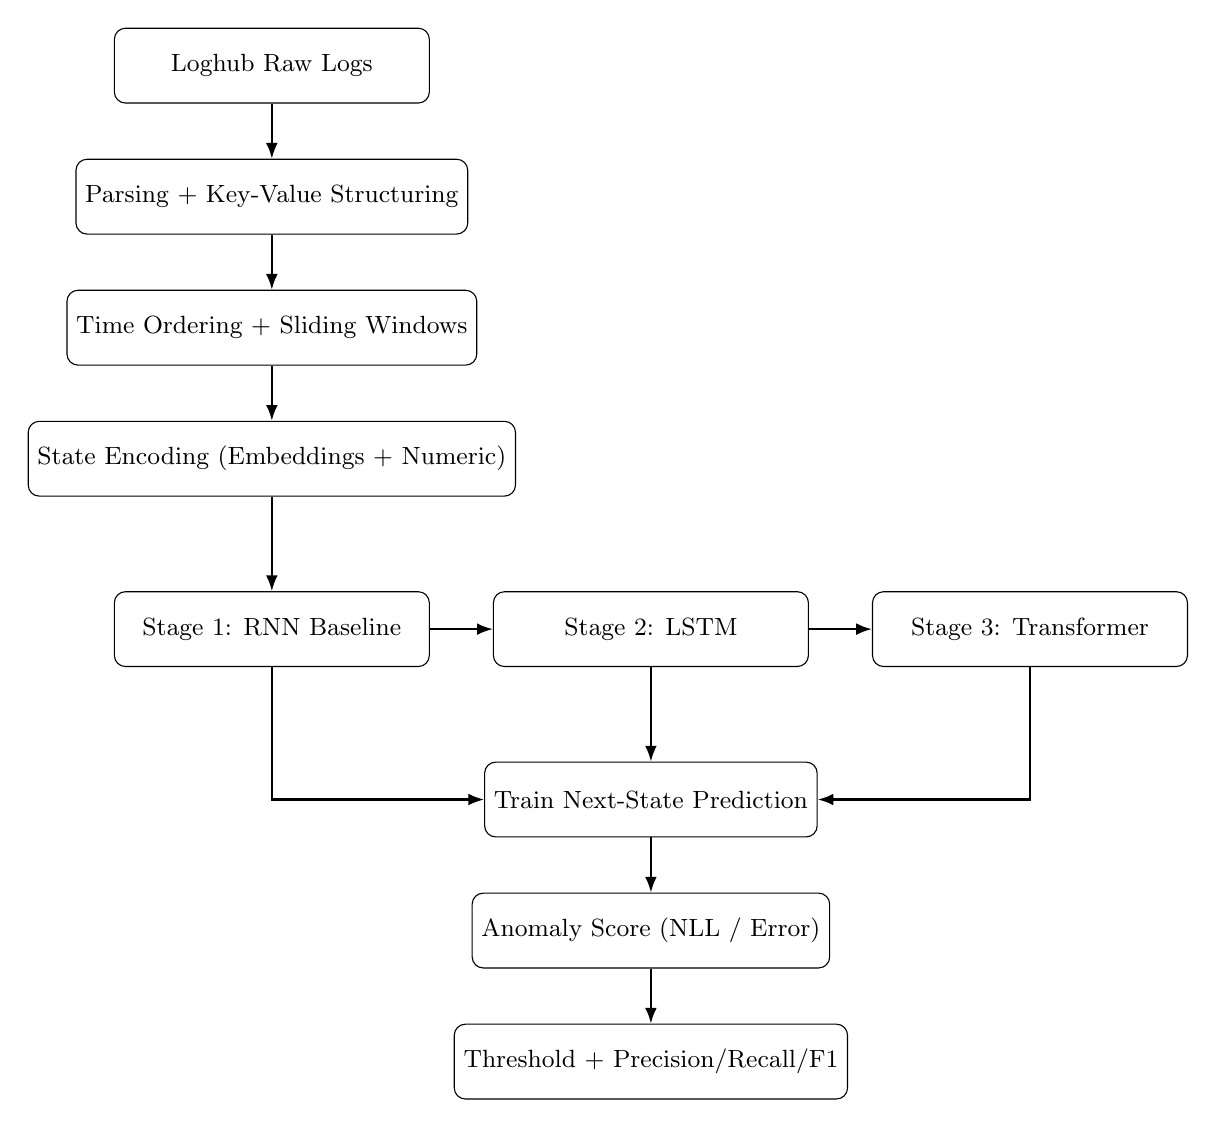
\begin{tikzpicture}[
    node distance=7mm and 8mm,
    box/.style={draw, rounded corners, align=center, minimum width=4.0cm, minimum height=0.95cm, font=\small},
    arrow/.style={-{Latex[length=2.0mm]}, thick}
]
\node[box, anchor=west] (data) at (0,0) {Loghub Raw Logs};
\node[box, below=of data] (prep) {Parsing + Key-Value Structuring};
\node[box, below=of prep] (seq) {Time Ordering + Sliding Windows};
\node[box, below=of seq] (feat) {State Encoding (Embeddings + Numeric)};

\node[box, below=12mm of feat] (rnn) {Stage 1: RNN Baseline};
\node[box, right=of rnn] (lstm) {Stage 2: LSTM};
\node[box, right=of lstm] (trf) {Stage 3: Transformer};

\node[box, below=12mm of lstm] (train) {Train Next-State Prediction};
\node[box, below=of train] (score) {Anomaly Score (NLL / Error)};
\node[box, below=of score] (eval) {Threshold + Precision/Recall/F1};

\draw[arrow] (data) -- (prep);
\draw[arrow] (prep) -- (seq);
\draw[arrow] (seq) -- (feat);
\draw[arrow] (feat) -- (rnn);
\draw[arrow] (rnn) -- (lstm);
\draw[arrow] (lstm) -- (trf);
\draw[arrow] (rnn) |- (train.west);
\draw[arrow] (lstm) -- (train);
\draw[arrow] (trf) |- (train.east);
\draw[arrow] (train) -- (score);
\draw[arrow] (score) -- (eval);
\end{tikzpicture}%
}
\end{center}

\section{Baseline Results}

As a baseline, we implement a vanilla Recurrent Neural Network (RNN) model to learn sequential patterns in log data. Each log entry is represented using a tokenized event template or structured encoding, and sequences are constructed using a fixed-length sliding window over time-ordered logs.

The RNN model is trained to predict the next log event given a sequence of previous events. The anomaly score is computed as the negative log-probability of the observed next event. Events that receive low probability under the trained model are flagged as anomalous.

The baseline model is evaluated using both prediction and anomaly detection metrics. For next-event prediction, we report accuracy and cross-entropy loss. For anomaly detection, we use precision, recall, and F1-score based on labeled anomalies available in the dataset.

Preliminary results indicate that the RNN is able to capture short-term sequential dependencies in log data and detect simple anomalies based on deviations from expected transitions. However, the model is limited in its ability to capture long-range dependencies and complex interactions across distant events in the sequence.

This baseline serves as a reference point for evaluating more advanced sequence modeling approaches.

\section{Technical Specification}

\textbf{Dataset:}
We use structured log data from the Loghub repository, specifically the OpenStack dataset. The logs are preprocessed into structured format with event templates and timestamps. Sequences are constructed using sliding windows over time-ordered log entries.

\textbf{Hardware:}
Experiments are conducted on a MacBook Pro with Apple M4 Pro chip and 16GB unified memory. Training is performed using CPU and Apple’s Metal Performance Shaders (MPS) backend for GPU acceleration where available.

\textbf{Software:}
\begin{itemize}
    \item Python 3.10
    \item PyTorch (for model implementation)
    \item NumPy and Pandas (for data processing)
    \item Scikit-learn (for evaluation metrics)
\end{itemize}

\textbf{Model Architecture (Baseline RNN):}
\begin{itemize}
    \item Embedding dimension: 32
    \item Hidden dimension: 64
    \item RNN type: Vanilla RNN
    \item Output layer: Fully connected (Linear) layer with softmax
\end{itemize}

\textbf{Training Configuration:}
\begin{itemize}
    \item Sequence length: 10
    \item Batch size: 32
    \item Learning rate: 0.001
    \item Optimizer: Adam
    \item Loss function: Cross-entropy loss
    \item Number of epochs: 5--10
\end{itemize}

\textbf{Evaluation Metrics:}
\begin{itemize}
    \item Prediction: Accuracy, Cross-Entropy Loss
    \item Anomaly Detection: Precision, Recall, F1-score
\end{itemize}

\textbf{Proposed Extension:}
To improve upon the baseline, we propose replacing the RNN with a Transformer-based model. The Transformer leverages self-attention to model relationships between all events in a sequence, allowing it to capture long-range dependencies and complex interactions more effectively than RNNs.


\begin{thebibliography}{10}

\bibitem{chandola2009survey}
V. Chandola et al.,
``Anomaly Detection: A Survey,'' 2009.

\bibitem{xu2009consolelogs}
W. Xu et al.,
``Detecting Large-Scale System Problems by Mining Console Logs,'' 2009.

\bibitem{lou2010invariants}
J. Lou et al.,
``Mining Invariants from Console Logs,'' 2010.

\bibitem{du2017deeplog}
M. Du et al.,
``DeepLog,'' 2017.

\bibitem{meng2019loganomaly}
W. Meng et al.,
``LogAnomaly,'' 2019.

\bibitem{guo2021logbert}
H. Guo et al.,
``LogBERT,'' 2021.

\bibitem{catillo2022autolog}
M. Catillo et al.,
``AutoLog,'' 2022.

\bibitem{li2024logs2graphs}
Z. Li et al.,
``Graph Neural Networks for Log Anomaly Detection,'' 2024.

\bibitem{landauer2023dlsurvey}
M. Landauer et al.,
``Deep Learning for Log Anomaly Detection,'' 2023.

\bibitem{loghub}
Loghub Dataset,
\url{https://github.com/logpai/loghub}

\end{thebibliography}

\end{document}